\newpage
\section{Projektowanie}
%Opis przygotowania narzędzi (git, visual studio). Wybór i opis bibliotek, klas. Szkic layoutów. Pseudo kody. Opisy wykorzystanych algorytmów (np. algorytm sortowania). Dokładniejsze określenie założeń i działania aplikacji, (np.: ten przycisk otworzy takie okno a w tym oknie wpisujemy takie dane).
\subsection{Przygotowanie narzędzi}

W ramach przygotowania środowiska do implementacji aplikacji wirtualnego dziekanatu oraz zarządzania wersjami kodu, wybrano zestaw narzędzi wspierających proces tworzenia oraz zapewniających automatyzację wielu czynności. W poniższych punktach opisano każde z wykorzystanych narzędzi wraz z ich rolą oraz załączonym linkiem do dokumentacji.

\begin{itemize}
  \item \textbf{Git} – system kontroli wersji, umożliwiający śledzenie zmian w kodzie oraz współpracę w zespole. Dokumentacja narzędzia: \url{https://git-scm.com/doc}
  \item \textbf{VSCode} – edytor kodu źródłowego, który zapewnia wsparcie dla wielu języków programowania i umożliwia instalację rozszerzeń wspierających programowanie. Dokumentacja narzędzia: \url{https://code.visualstudio.com/docs}
  \item \textbf{Android Studio} – środowisko programistyczne wykorzystywane głównie do testowania aplikacji na emulatorze Android oraz zarządzania SDK. Dokumentacja: \url{https://developer.android.com/studio/intro}
  \item \textbf{Flutter SDK} – zestaw narzędzi do tworzenia aplikacji wieloplatformowych. Dokumentacja: \url{https://flutter.dev/docs}
  \item \textbf{Doxygen} – narzędzie do generowania dokumentacji automatycznej na podstawie komentarzy w kodzie źródłowym. Dokumentacja narzędzia: \url{https://www.doxygen.nl/}
  \item \textbf{Doxygen Awesome} – motyw graficzny dostosowujący wygląd strony wygenerowanej przez Doxygen do współczesnych standardów. Więcej informacji: \url{https://github.com/jothepro/doxygen-awesome-css}
  \item \textbf{Lefthook} – narzędzie do zarządzania hookami Git, które wspiera automatyczne formatowanie, walidację kodu oraz zgodność wiadomości commitów z konwencją. Dokumentacja: \url{https://github.com/evilmartians/lefthook}
  \item \textbf{Commitlint} – narzędzie do sprawdzania zgodności wiadomości commitów z konwencją \textit{Conventional Commits}. Dokumentacja: \url{https://commitlint.js.org/}
  \item \textbf{GitHub Actions} – platforma do automatyzacji procesów CI/CD. Umożliwia automatyczną walidację commitów, generowanie dokumentacji oraz wersjonowanie wydań. Dokumentacja: \url{https://docs.github.com/en/actions}
\end{itemize}

\subsection{Architektura systemu}

Aplikacja została zbudowana w oparciu o dwa główne komponenty:

\begin{itemize}
  \item \textbf{Backend - Payload CMS} – główny system zarządzania treścią, odpowiedzialny za:
        \begin{itemize}
          \item Autoryzację i uwierzytelnianie użytkowników
          \item Przechowywanie i zarządzanie danymi aplikacji
          \item API REST do komunikacji z aplikacją mobilną
          \item Panel administracyjny dla pracowników uczelni
        \end{itemize}

  \item \textbf{Firebase Cloud Messaging} – wykorzystywany wyłącznie do obsługi powiadomień push:
        \begin{itemize}
          \item Wysyłanie powiadomień o zmianach w planie zajęć
          \item Informowanie o nowych ogłoszeniach
          \item Powiadomienia o nowych wiadomościach
        \end{itemize}
\end{itemize}

\subsection{Framework Flutter}
System składa się z trzech głównych komponentów:

\begin{figure}[h]
  \centering
  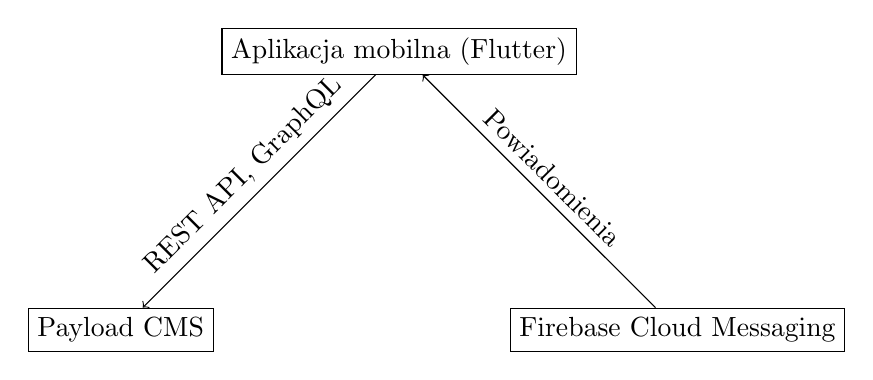
\begin{tikzpicture}[node distance=5cm]
    \node[draw,rectangle] (app) {Aplikacja mobilna (Flutter)};
    \node[draw,rectangle] (cms) [below left of=app] {Payload CMS};
    \node[draw,rectangle] (fcm) [below right of=app] {Firebase Cloud Messaging};
    \draw[->] (app) -- (cms) node[midway,above,sloped] {REST API, GraphQL};
    \draw[->] (fcm) -- (app) node[midway,above,sloped] {Powiadomienia};
  \end{tikzpicture}
  \caption{Architektura systemu}
  \label{fig:architecture}
\end{figure}
\newpage
\subsection{Architektura systemu}
Architektura aplikacji została zaprojektowana w modelu klient-serwer z następującymi komponentami:

\begin{itemize}
  \item \textbf{Frontend (aplikacja mobilna)}:
        \begin{itemize}
          \item Interfejs użytkownika w Material Design
          \item Zarządzanie stanem aplikacji (Riverpod)
          \item Przechowywanie danych lokalnych
          \item Obsługa trybu offline
        \end{itemize}

  \item \textbf{Backend (Payload CMS)}:
        \begin{itemize}
          \item REST API
          \item System autoryzacji
          \item Baza danych
          \item Panel administracyjny
          \item GraphQL
        \end{itemize}

  \item \textbf{Usługi zewnętrzne}:
        \begin{itemize}
          \item Firebase Cloud Messaging (powiadomienia push)
        \end{itemize}
\end{itemize}

\subsection{Projekt interfejsu użytkownika}

\subsubsection{Style i motywy}
\begin{itemize}
  \item Spójny system projektowy Material Design 3
  \item Wsparcie dla motywu jasnego i ciemnego
  \item Dynamiczne dostosowanie do różnych rozmiarów ekranów
  \item Responsywne komponenty UI
\end{itemize}

\subsubsection{Nawigacja}
\begin{itemize}
  \item Menu dolne z 4 głównymi sekcjami:
        \begin{itemize}
          \item Panel główny
          \item Powiadomienia
          \item Wiadomości
          \item Ustawienia
        \end{itemize}
  \item Nawigacja stosowa między ekranami
  \item Gesty nawigacyjne (swipe)
\end{itemize}

\subsection{Model danych}

\subsubsection{Główne encje}
\begin{itemize}
  \item \textbf{User}:
        \begin{itemize}
          \item Dane podstawowe (imię, nazwisko, email)
          \item Rola (student/wykładowca/admin)
          \item Ustawienia (język, powiadomienia)
        \end{itemize}

  \item \textbf{Schedule}:
        \begin{itemize}
          \item Przedmiot
          \item Data i czas
          \item Sala
          \item Prowadzący
        \end{itemize}

  \item \textbf{Notification}:
        \begin{itemize}
          \item Typ
          \item Treść
          \item Data
          \item Odbiorcy
        \end{itemize}
\end{itemize}

\subsection{Bezpieczeństwo}

\begin{itemize}
  \item \textbf{Autoryzacja}:
        \begin{itemize}
          \item JWT tokens
          \item Refresh tokens
          \item Szyfrowanie danych wrażliwych
        \end{itemize}

  \item \textbf{Walidacja danych}:
        \begin{itemize}
          \item Walidacja formularzy
          \item Sanityzacja danych wejściowych
          \item Obsługa błędów
        \end{itemize}
\end{itemize}

\subsection{Synchronizacja danych}

\begin{itemize}
  \item \textbf{Cache lokalny}:
        \begin{itemize}
          \item Przechowywanie planu zajęć
          \item Buforowanie ogłoszeń
          \item Ustawienia użytkownika
        \end{itemize}

  \item \textbf{Strategia synchronizacji}:
        \begin{itemize}
          \item Automatyczna synchronizacja w tle
          \item Ręczne odświeżanie danych
          \item Kolejkowanie operacji offline
        \end{itemize}
\end{itemize}
\subsection{Diagram UML}
% Klasa Student
\begin{figure}[H]
  \centering
  \begin{tikzpicture}
    \umlclass[x=0, y=0]{Student}{
      - id: int \\
      - firstName: String \\
      - middleName: dynamic \\
      - familyName: String \\
      - coursesOfStudy: List<CoursesOfStudy> \\
      - dateOfBirth: DateTime \\
      - updatedAt: DateTime \\
      - createdAt: DateTime \\
      - collection: String \\
      - loginAttempts: int
    }{
      + factory Student.fromJson(Map<String, dynamic> json) \\
      + toJson(): Map<String, dynamic>
    }
  \end{tikzpicture}
  \caption{Klasa Student}
  \label{fig:class-student}
\end{figure}
\newpage
% Klasa Schedule
\begin{figure}[H]
  \centering
  \begin{tikzpicture}
    \umlclass[x=0, y=0]{Schedule}{
      - id: int \\
      - courseOfStudy: int \\
      - weekAfullTimeSchedule: WeekFullTimeSchedule \\
      - weekAPartTimeSchedule: WeekPartTimeSchedule \\
      - weekBfullTimeSchedule: WeekFullTimeSchedule \\
      - weekBPartTimeSchedule: WeekPartTimeSchedule \\
      - updatedAt: DateTime \\
      - createdAt: DateTime
    }{
      + factory Schedule.fromJson(Map<String, dynamic> json) \\
      + toJson(): Map<String, dynamic>
    }
  \end{tikzpicture}
  \caption{Klasa Schedule}
  \label{fig:class-schedule}
\end{figure}

% Klasa CoursesOfStudy
\begin{figure}[H]
  \centering
  \begin{tikzpicture}
    \umlclass[x=0, y=0]{CoursesOfStudy}{
      - id: int \\
      - fieldOfStudy: String \\
      - faculty: Faculty \\
      - schedule: Schedule \\
      - courseType: String \\
      - levelOfStudy: String \\
      - obtainedTitle: String \\
      - numberOfSemesters: int \\
      - currentSemester: int \\
      - startDate: DateTime \\
      - endDate: DateTime \\
      - updatedAt: DateTime \\
      - createdAt: DateTime
    }{
      + factory CoursesOfStudy.fromJson(Map<String, dynamic> json) \\
      + toJson(): Map<String, dynamic>
    }
  \end{tikzpicture}
  \caption{Klasa CoursesOfStudy}
  \label{fig:class-coursesofstudy}
\end{figure}
